% ---------
%  Compile with "pdflatex hw0".
% --------
%!TEX TS-program = pdflatex
%!TEX encoding = UTF-8 Unicode

\documentclass[11pt]{article}
\usepackage{jeffe,handout,graphicx}
\usepackage[utf8]{inputenc}		% Allow some non-ASCII Unicode in source

%  Redefine suits
\usepackage{pifont}
\def\Spade{\text{\ding{171}}}
\def\Heart{\text{\textcolor{Red}{\ding{170}}}}
\def\Diamond{\text{\textcolor{Red}{\ding{169}}}}
\def\Club{\text{\ding{168}}}

\def\Cdot{\mathbin{\text{\normalfont \textbullet}}}
\def\Sym#1{\textbf{\texttt{\color{BrickRed}#1}}}



% =====================================================
%   Define common stuff for solution headers
% =====================================================
\Class{CS $498$ algorithm}
\Semester{Spring $2019$}
\Authors{2}
%\Section{}

% =====================================================
\begin{document}

% ---------------------------------------------------------


% ---------------------------------------------------------
% Change authors again
\AuthorOne{Ray Ying}{xinruiy2@illinois.edu}
\AuthorTwo{Aditya Pillai}{apillai4@illinois.edu}

\HomeworkHeader{$2$}{$1$}

\begin{quote}

\end{quote}
\hrule


\begin{solution}
\item
\begin{enumerate}
    \item   I choose python to implement the counters. Given a list of items, integers in my case, and count the length of the list. Whenever a new integer comes, I randomly select $1$ number from a list from $0$ to $2^{X}$ or $(1+a)^{X}$, only increases the counter $X$ when the number selected is $0$.\\
    I made $8$ copies , $a = 3$,  $\epsilon = 1/2$, and $\delta = 1/8$. 
    \item The plot of $n = 2^{16}$ to the three counters(I did eight times corresponding to the $x$ axis):\\
    \\
    \begin{figure}[h]
    \centering
    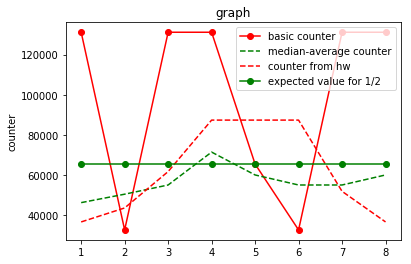
\includegraphics[width=1\textwidth]{hw2/counters.png}
    \caption{n and three counters}
    \end{figure}
    \newpage
    The plot of $n$ comparing to the needed bits($x$ is the log of the length of the array):\\
    \begin{figure}[h]
    \centering
    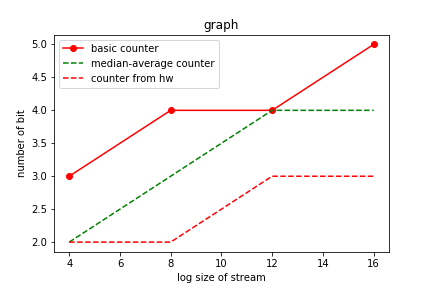
\includegraphics[width=1\textwidth]{hw2/pic.png}
    \caption{n with the bit needed}
    \end{figure}
    \\
    \item Comparing to the theoretical space, my implementation will need extra space for the step of "flip biased coins", an array of size of minimum $2^X$ or $(1+a)^{X}$ for it. Also, my code didn't implement a bit counter. \\
    The performance is pretty accurate to the expectation, when doing the basic counter, the value is pretty inaccurate due to the large variance. After doing the average and median trick, the expected success rate that the value is in the range of $\epsilon = 1/2$ times the length of the array should be $1- \delta = 7/8$ and the success rate in my experiment is just $7/8$. When I use the way describe in the homework, the number of bits required reduce but it seems less reliable than using $(1/2^x)$ rather than $1/(1+a)^x$ with higher variance.\\
    Also, when given the string length too big, the computer is really hard and slow at computing the counter especially with average and median tricks. 
    
\end{enumerate}

\end{solution}
\end{document}
